
% Default to the notebook output style

    


% Inherit from the specified cell style.




    
\documentclass[11pt]{article}

    
    
    \usepackage[T1]{fontenc}
    % Nicer default font (+ math font) than Computer Modern for most use cases
    \usepackage{mathpazo}

    % Basic figure setup, for now with no caption control since it's done
    % automatically by Pandoc (which extracts ![](path) syntax from Markdown).
    \usepackage{graphicx}
    % We will generate all images so they have a width \maxwidth. This means
    % that they will get their normal width if they fit onto the page, but
    % are scaled down if they would overflow the margins.
    \makeatletter
    \def\maxwidth{\ifdim\Gin@nat@width>\linewidth\linewidth
    \else\Gin@nat@width\fi}
    \makeatother
    \let\Oldincludegraphics\includegraphics
    % Set max figure width to be 80% of text width, for now hardcoded.
    \renewcommand{\includegraphics}[1]{\Oldincludegraphics[width=.8\maxwidth]{#1}}
    % Ensure that by default, figures have no caption (until we provide a
    % proper Figure object with a Caption API and a way to capture that
    % in the conversion process - todo).
    \usepackage{caption}
    \DeclareCaptionLabelFormat{nolabel}{}
    \captionsetup{labelformat=nolabel}

    \usepackage{adjustbox} % Used to constrain images to a maximum size 
    \usepackage{xcolor} % Allow colors to be defined
    \usepackage{enumerate} % Needed for markdown enumerations to work
    \usepackage{geometry} % Used to adjust the document margins
    \usepackage{amsmath} % Equations
    \usepackage{amssymb} % Equations
    \usepackage{textcomp} % defines textquotesingle
    % Hack from http://tex.stackexchange.com/a/47451/13684:
    \AtBeginDocument{%
        \def\PYZsq{\textquotesingle}% Upright quotes in Pygmentized code
    }
    \usepackage{upquote} % Upright quotes for verbatim code
    \usepackage{eurosym} % defines \euro
    \usepackage[mathletters]{ucs} % Extended unicode (utf-8) support
    \usepackage[utf8x]{inputenc} % Allow utf-8 characters in the tex document
    \usepackage{fancyvrb} % verbatim replacement that allows latex
    \usepackage{grffile} % extends the file name processing of package graphics 
                         % to support a larger range 
    % The hyperref package gives us a pdf with properly built
    % internal navigation ('pdf bookmarks' for the table of contents,
    % internal cross-reference links, web links for URLs, etc.)
    \usepackage{hyperref}
    \usepackage{longtable} % longtable support required by pandoc >1.10
    \usepackage{booktabs}  % table support for pandoc > 1.12.2
    \usepackage[inline]{enumitem} % IRkernel/repr support (it uses the enumerate* environment)
    \usepackage[normalem]{ulem} % ulem is needed to support strikethroughs (\sout)
                                % normalem makes italics be italics, not underlines
    

    
    
    % Colors for the hyperref package
    \definecolor{urlcolor}{rgb}{0,.145,.698}
    \definecolor{linkcolor}{rgb}{.71,0.21,0.01}
    \definecolor{citecolor}{rgb}{.12,.54,.11}

    % ANSI colors
    \definecolor{ansi-black}{HTML}{3E424D}
    \definecolor{ansi-black-intense}{HTML}{282C36}
    \definecolor{ansi-red}{HTML}{E75C58}
    \definecolor{ansi-red-intense}{HTML}{B22B31}
    \definecolor{ansi-green}{HTML}{00A250}
    \definecolor{ansi-green-intense}{HTML}{007427}
    \definecolor{ansi-yellow}{HTML}{DDB62B}
    \definecolor{ansi-yellow-intense}{HTML}{B27D12}
    \definecolor{ansi-blue}{HTML}{208FFB}
    \definecolor{ansi-blue-intense}{HTML}{0065CA}
    \definecolor{ansi-magenta}{HTML}{D160C4}
    \definecolor{ansi-magenta-intense}{HTML}{A03196}
    \definecolor{ansi-cyan}{HTML}{60C6C8}
    \definecolor{ansi-cyan-intense}{HTML}{258F8F}
    \definecolor{ansi-white}{HTML}{C5C1B4}
    \definecolor{ansi-white-intense}{HTML}{A1A6B2}

    % commands and environments needed by pandoc snippets
    % extracted from the output of `pandoc -s`
    \providecommand{\tightlist}{%
      \setlength{\itemsep}{0pt}\setlength{\parskip}{0pt}}
    \DefineVerbatimEnvironment{Highlighting}{Verbatim}{commandchars=\\\{\}}
    % Add ',fontsize=\small' for more characters per line
    \newenvironment{Shaded}{}{}
    \newcommand{\KeywordTok}[1]{\textcolor[rgb]{0.00,0.44,0.13}{\textbf{{#1}}}}
    \newcommand{\DataTypeTok}[1]{\textcolor[rgb]{0.56,0.13,0.00}{{#1}}}
    \newcommand{\DecValTok}[1]{\textcolor[rgb]{0.25,0.63,0.44}{{#1}}}
    \newcommand{\BaseNTok}[1]{\textcolor[rgb]{0.25,0.63,0.44}{{#1}}}
    \newcommand{\FloatTok}[1]{\textcolor[rgb]{0.25,0.63,0.44}{{#1}}}
    \newcommand{\CharTok}[1]{\textcolor[rgb]{0.25,0.44,0.63}{{#1}}}
    \newcommand{\StringTok}[1]{\textcolor[rgb]{0.25,0.44,0.63}{{#1}}}
    \newcommand{\CommentTok}[1]{\textcolor[rgb]{0.38,0.63,0.69}{\textit{{#1}}}}
    \newcommand{\OtherTok}[1]{\textcolor[rgb]{0.00,0.44,0.13}{{#1}}}
    \newcommand{\AlertTok}[1]{\textcolor[rgb]{1.00,0.00,0.00}{\textbf{{#1}}}}
    \newcommand{\FunctionTok}[1]{\textcolor[rgb]{0.02,0.16,0.49}{{#1}}}
    \newcommand{\RegionMarkerTok}[1]{{#1}}
    \newcommand{\ErrorTok}[1]{\textcolor[rgb]{1.00,0.00,0.00}{\textbf{{#1}}}}
    \newcommand{\NormalTok}[1]{{#1}}
    
    % Additional commands for more recent versions of Pandoc
    \newcommand{\ConstantTok}[1]{\textcolor[rgb]{0.53,0.00,0.00}{{#1}}}
    \newcommand{\SpecialCharTok}[1]{\textcolor[rgb]{0.25,0.44,0.63}{{#1}}}
    \newcommand{\VerbatimStringTok}[1]{\textcolor[rgb]{0.25,0.44,0.63}{{#1}}}
    \newcommand{\SpecialStringTok}[1]{\textcolor[rgb]{0.73,0.40,0.53}{{#1}}}
    \newcommand{\ImportTok}[1]{{#1}}
    \newcommand{\DocumentationTok}[1]{\textcolor[rgb]{0.73,0.13,0.13}{\textit{{#1}}}}
    \newcommand{\AnnotationTok}[1]{\textcolor[rgb]{0.38,0.63,0.69}{\textbf{\textit{{#1}}}}}
    \newcommand{\CommentVarTok}[1]{\textcolor[rgb]{0.38,0.63,0.69}{\textbf{\textit{{#1}}}}}
    \newcommand{\VariableTok}[1]{\textcolor[rgb]{0.10,0.09,0.49}{{#1}}}
    \newcommand{\ControlFlowTok}[1]{\textcolor[rgb]{0.00,0.44,0.13}{\textbf{{#1}}}}
    \newcommand{\OperatorTok}[1]{\textcolor[rgb]{0.40,0.40,0.40}{{#1}}}
    \newcommand{\BuiltInTok}[1]{{#1}}
    \newcommand{\ExtensionTok}[1]{{#1}}
    \newcommand{\PreprocessorTok}[1]{\textcolor[rgb]{0.74,0.48,0.00}{{#1}}}
    \newcommand{\AttributeTok}[1]{\textcolor[rgb]{0.49,0.56,0.16}{{#1}}}
    \newcommand{\InformationTok}[1]{\textcolor[rgb]{0.38,0.63,0.69}{\textbf{\textit{{#1}}}}}
    \newcommand{\WarningTok}[1]{\textcolor[rgb]{0.38,0.63,0.69}{\textbf{\textit{{#1}}}}}
    
    
    % Define a nice break command that doesn't care if a line doesn't already
    % exist.
    \def\br{\hspace*{\fill} \\* }
    % Math Jax compatability definitions
    \def\gt{>}
    \def\lt{<}
    % Document parameters
    \title{Gentle Introduction to GPU Programming in Numba}
    
    
    

    % Pygments definitions
    
\makeatletter
\def\PY@reset{\let\PY@it=\relax \let\PY@bf=\relax%
    \let\PY@ul=\relax \let\PY@tc=\relax%
    \let\PY@bc=\relax \let\PY@ff=\relax}
\def\PY@tok#1{\csname PY@tok@#1\endcsname}
\def\PY@toks#1+{\ifx\relax#1\empty\else%
    \PY@tok{#1}\expandafter\PY@toks\fi}
\def\PY@do#1{\PY@bc{\PY@tc{\PY@ul{%
    \PY@it{\PY@bf{\PY@ff{#1}}}}}}}
\def\PY#1#2{\PY@reset\PY@toks#1+\relax+\PY@do{#2}}

\expandafter\def\csname PY@tok@vi\endcsname{\def\PY@tc##1{\textcolor[rgb]{0.10,0.09,0.49}{##1}}}
\expandafter\def\csname PY@tok@c\endcsname{\let\PY@it=\textit\def\PY@tc##1{\textcolor[rgb]{0.25,0.50,0.50}{##1}}}
\expandafter\def\csname PY@tok@sx\endcsname{\def\PY@tc##1{\textcolor[rgb]{0.00,0.50,0.00}{##1}}}
\expandafter\def\csname PY@tok@nt\endcsname{\let\PY@bf=\textbf\def\PY@tc##1{\textcolor[rgb]{0.00,0.50,0.00}{##1}}}
\expandafter\def\csname PY@tok@w\endcsname{\def\PY@tc##1{\textcolor[rgb]{0.73,0.73,0.73}{##1}}}
\expandafter\def\csname PY@tok@mi\endcsname{\def\PY@tc##1{\textcolor[rgb]{0.40,0.40,0.40}{##1}}}
\expandafter\def\csname PY@tok@mb\endcsname{\def\PY@tc##1{\textcolor[rgb]{0.40,0.40,0.40}{##1}}}
\expandafter\def\csname PY@tok@kp\endcsname{\def\PY@tc##1{\textcolor[rgb]{0.00,0.50,0.00}{##1}}}
\expandafter\def\csname PY@tok@sa\endcsname{\def\PY@tc##1{\textcolor[rgb]{0.73,0.13,0.13}{##1}}}
\expandafter\def\csname PY@tok@gs\endcsname{\let\PY@bf=\textbf}
\expandafter\def\csname PY@tok@nn\endcsname{\let\PY@bf=\textbf\def\PY@tc##1{\textcolor[rgb]{0.00,0.00,1.00}{##1}}}
\expandafter\def\csname PY@tok@nv\endcsname{\def\PY@tc##1{\textcolor[rgb]{0.10,0.09,0.49}{##1}}}
\expandafter\def\csname PY@tok@mh\endcsname{\def\PY@tc##1{\textcolor[rgb]{0.40,0.40,0.40}{##1}}}
\expandafter\def\csname PY@tok@ge\endcsname{\let\PY@it=\textit}
\expandafter\def\csname PY@tok@s\endcsname{\def\PY@tc##1{\textcolor[rgb]{0.73,0.13,0.13}{##1}}}
\expandafter\def\csname PY@tok@go\endcsname{\def\PY@tc##1{\textcolor[rgb]{0.53,0.53,0.53}{##1}}}
\expandafter\def\csname PY@tok@fm\endcsname{\def\PY@tc##1{\textcolor[rgb]{0.00,0.00,1.00}{##1}}}
\expandafter\def\csname PY@tok@kt\endcsname{\def\PY@tc##1{\textcolor[rgb]{0.69,0.00,0.25}{##1}}}
\expandafter\def\csname PY@tok@ne\endcsname{\let\PY@bf=\textbf\def\PY@tc##1{\textcolor[rgb]{0.82,0.25,0.23}{##1}}}
\expandafter\def\csname PY@tok@se\endcsname{\let\PY@bf=\textbf\def\PY@tc##1{\textcolor[rgb]{0.73,0.40,0.13}{##1}}}
\expandafter\def\csname PY@tok@nd\endcsname{\def\PY@tc##1{\textcolor[rgb]{0.67,0.13,1.00}{##1}}}
\expandafter\def\csname PY@tok@no\endcsname{\def\PY@tc##1{\textcolor[rgb]{0.53,0.00,0.00}{##1}}}
\expandafter\def\csname PY@tok@gh\endcsname{\let\PY@bf=\textbf\def\PY@tc##1{\textcolor[rgb]{0.00,0.00,0.50}{##1}}}
\expandafter\def\csname PY@tok@gu\endcsname{\let\PY@bf=\textbf\def\PY@tc##1{\textcolor[rgb]{0.50,0.00,0.50}{##1}}}
\expandafter\def\csname PY@tok@vc\endcsname{\def\PY@tc##1{\textcolor[rgb]{0.10,0.09,0.49}{##1}}}
\expandafter\def\csname PY@tok@sh\endcsname{\def\PY@tc##1{\textcolor[rgb]{0.73,0.13,0.13}{##1}}}
\expandafter\def\csname PY@tok@o\endcsname{\def\PY@tc##1{\textcolor[rgb]{0.40,0.40,0.40}{##1}}}
\expandafter\def\csname PY@tok@kd\endcsname{\let\PY@bf=\textbf\def\PY@tc##1{\textcolor[rgb]{0.00,0.50,0.00}{##1}}}
\expandafter\def\csname PY@tok@nl\endcsname{\def\PY@tc##1{\textcolor[rgb]{0.63,0.63,0.00}{##1}}}
\expandafter\def\csname PY@tok@bp\endcsname{\def\PY@tc##1{\textcolor[rgb]{0.00,0.50,0.00}{##1}}}
\expandafter\def\csname PY@tok@c1\endcsname{\let\PY@it=\textit\def\PY@tc##1{\textcolor[rgb]{0.25,0.50,0.50}{##1}}}
\expandafter\def\csname PY@tok@vg\endcsname{\def\PY@tc##1{\textcolor[rgb]{0.10,0.09,0.49}{##1}}}
\expandafter\def\csname PY@tok@gi\endcsname{\def\PY@tc##1{\textcolor[rgb]{0.00,0.63,0.00}{##1}}}
\expandafter\def\csname PY@tok@vm\endcsname{\def\PY@tc##1{\textcolor[rgb]{0.10,0.09,0.49}{##1}}}
\expandafter\def\csname PY@tok@gd\endcsname{\def\PY@tc##1{\textcolor[rgb]{0.63,0.00,0.00}{##1}}}
\expandafter\def\csname PY@tok@gt\endcsname{\def\PY@tc##1{\textcolor[rgb]{0.00,0.27,0.87}{##1}}}
\expandafter\def\csname PY@tok@kn\endcsname{\let\PY@bf=\textbf\def\PY@tc##1{\textcolor[rgb]{0.00,0.50,0.00}{##1}}}
\expandafter\def\csname PY@tok@sb\endcsname{\def\PY@tc##1{\textcolor[rgb]{0.73,0.13,0.13}{##1}}}
\expandafter\def\csname PY@tok@mf\endcsname{\def\PY@tc##1{\textcolor[rgb]{0.40,0.40,0.40}{##1}}}
\expandafter\def\csname PY@tok@na\endcsname{\def\PY@tc##1{\textcolor[rgb]{0.49,0.56,0.16}{##1}}}
\expandafter\def\csname PY@tok@k\endcsname{\let\PY@bf=\textbf\def\PY@tc##1{\textcolor[rgb]{0.00,0.50,0.00}{##1}}}
\expandafter\def\csname PY@tok@kc\endcsname{\let\PY@bf=\textbf\def\PY@tc##1{\textcolor[rgb]{0.00,0.50,0.00}{##1}}}
\expandafter\def\csname PY@tok@err\endcsname{\def\PY@bc##1{\setlength{\fboxsep}{0pt}\fcolorbox[rgb]{1.00,0.00,0.00}{1,1,1}{\strut ##1}}}
\expandafter\def\csname PY@tok@s1\endcsname{\def\PY@tc##1{\textcolor[rgb]{0.73,0.13,0.13}{##1}}}
\expandafter\def\csname PY@tok@si\endcsname{\let\PY@bf=\textbf\def\PY@tc##1{\textcolor[rgb]{0.73,0.40,0.53}{##1}}}
\expandafter\def\csname PY@tok@kr\endcsname{\let\PY@bf=\textbf\def\PY@tc##1{\textcolor[rgb]{0.00,0.50,0.00}{##1}}}
\expandafter\def\csname PY@tok@ss\endcsname{\def\PY@tc##1{\textcolor[rgb]{0.10,0.09,0.49}{##1}}}
\expandafter\def\csname PY@tok@nb\endcsname{\def\PY@tc##1{\textcolor[rgb]{0.00,0.50,0.00}{##1}}}
\expandafter\def\csname PY@tok@ch\endcsname{\let\PY@it=\textit\def\PY@tc##1{\textcolor[rgb]{0.25,0.50,0.50}{##1}}}
\expandafter\def\csname PY@tok@sc\endcsname{\def\PY@tc##1{\textcolor[rgb]{0.73,0.13,0.13}{##1}}}
\expandafter\def\csname PY@tok@cpf\endcsname{\let\PY@it=\textit\def\PY@tc##1{\textcolor[rgb]{0.25,0.50,0.50}{##1}}}
\expandafter\def\csname PY@tok@gr\endcsname{\def\PY@tc##1{\textcolor[rgb]{1.00,0.00,0.00}{##1}}}
\expandafter\def\csname PY@tok@il\endcsname{\def\PY@tc##1{\textcolor[rgb]{0.40,0.40,0.40}{##1}}}
\expandafter\def\csname PY@tok@gp\endcsname{\let\PY@bf=\textbf\def\PY@tc##1{\textcolor[rgb]{0.00,0.00,0.50}{##1}}}
\expandafter\def\csname PY@tok@ow\endcsname{\let\PY@bf=\textbf\def\PY@tc##1{\textcolor[rgb]{0.67,0.13,1.00}{##1}}}
\expandafter\def\csname PY@tok@ni\endcsname{\let\PY@bf=\textbf\def\PY@tc##1{\textcolor[rgb]{0.60,0.60,0.60}{##1}}}
\expandafter\def\csname PY@tok@nf\endcsname{\def\PY@tc##1{\textcolor[rgb]{0.00,0.00,1.00}{##1}}}
\expandafter\def\csname PY@tok@cp\endcsname{\def\PY@tc##1{\textcolor[rgb]{0.74,0.48,0.00}{##1}}}
\expandafter\def\csname PY@tok@cs\endcsname{\let\PY@it=\textit\def\PY@tc##1{\textcolor[rgb]{0.25,0.50,0.50}{##1}}}
\expandafter\def\csname PY@tok@sr\endcsname{\def\PY@tc##1{\textcolor[rgb]{0.73,0.40,0.53}{##1}}}
\expandafter\def\csname PY@tok@mo\endcsname{\def\PY@tc##1{\textcolor[rgb]{0.40,0.40,0.40}{##1}}}
\expandafter\def\csname PY@tok@nc\endcsname{\let\PY@bf=\textbf\def\PY@tc##1{\textcolor[rgb]{0.00,0.00,1.00}{##1}}}
\expandafter\def\csname PY@tok@dl\endcsname{\def\PY@tc##1{\textcolor[rgb]{0.73,0.13,0.13}{##1}}}
\expandafter\def\csname PY@tok@sd\endcsname{\let\PY@it=\textit\def\PY@tc##1{\textcolor[rgb]{0.73,0.13,0.13}{##1}}}
\expandafter\def\csname PY@tok@cm\endcsname{\let\PY@it=\textit\def\PY@tc##1{\textcolor[rgb]{0.25,0.50,0.50}{##1}}}
\expandafter\def\csname PY@tok@m\endcsname{\def\PY@tc##1{\textcolor[rgb]{0.40,0.40,0.40}{##1}}}
\expandafter\def\csname PY@tok@s2\endcsname{\def\PY@tc##1{\textcolor[rgb]{0.73,0.13,0.13}{##1}}}

\def\PYZbs{\char`\\}
\def\PYZus{\char`\_}
\def\PYZob{\char`\{}
\def\PYZcb{\char`\}}
\def\PYZca{\char`\^}
\def\PYZam{\char`\&}
\def\PYZlt{\char`\<}
\def\PYZgt{\char`\>}
\def\PYZsh{\char`\#}
\def\PYZpc{\char`\%}
\def\PYZdl{\char`\$}
\def\PYZhy{\char`\-}
\def\PYZsq{\char`\'}
\def\PYZdq{\char`\"}
\def\PYZti{\char`\~}
% for compatibility with earlier versions
\def\PYZat{@}
\def\PYZlb{[}
\def\PYZrb{]}
\makeatother


    % Exact colors from NB
    \definecolor{incolor}{rgb}{0.0, 0.0, 0.5}
    \definecolor{outcolor}{rgb}{0.545, 0.0, 0.0}



    
    % Prevent overflowing lines due to hard-to-break entities
    \sloppy 
    % Setup hyperref package
    \hypersetup{
      breaklinks=true,  % so long urls are correctly broken across lines
      colorlinks=true,
      urlcolor=urlcolor,
      linkcolor=linkcolor,
      citecolor=citecolor,
      }
    % Slightly bigger margins than the latex defaults
    
    \geometry{verbose,tmargin=1in,bmargin=1in,lmargin=1in,rmargin=1in}
    
    

    \begin{document}
    
    
    \maketitle
    
    

    
    \section{A Gentle Introduction to GPU Programming using
Numba}\label{a-gentle-introduction-to-gpu-programming-using-numba}

\begin{quote}
By Lokesh Kumar T
\end{quote}

\begin{quote}
Sept 2018
\end{quote}

\begin{quote}
IIT Madras
\end{quote}

    \section{Overview of the Talk}\label{overview-of-the-talk}

\begin{itemize}
\tightlist
\item
  CPUs and GPUs
\item
  Whats Heterogenous Computing?
\item
  Introduction to GPU Programming Terminologies
\item
  Introduction to Numba
\item
  Lets multiply a vector by 2 in GPU!
\item
  Matrix Multiplication in a GPU
\item
  How to proceed further?
\end{itemize}

    CPUs are generally increasingly good in reducing \emph{latency} for
single stream of processing.

\textbf{Fundamental performance quest in single core CPU:}

How to devote transistors on a chip to make a single stream of
instructions run faster and faster.

    \begin{itemize}
\tightlist
\item
  \textbf{CPU}: work on a variety of different calculations
\item
  \textbf{GPU}: best at focusing all the computing abilities on a
  specific task
\item
  \textbf{CPU}: few cores (up to 24) optimized for sequential serial
  processing
\item
  \textbf{GPU}: thousands of smaller and more efficient cores for a
  massively parallel architecture
\item
  \textbf{GPU}s provide \textbf{superior processing power},
  \textbf{memory bandwidth} and \textbf{efficiency} over their CPU
  counterparts.
\end{itemize}

    \begin{figure}
\centering
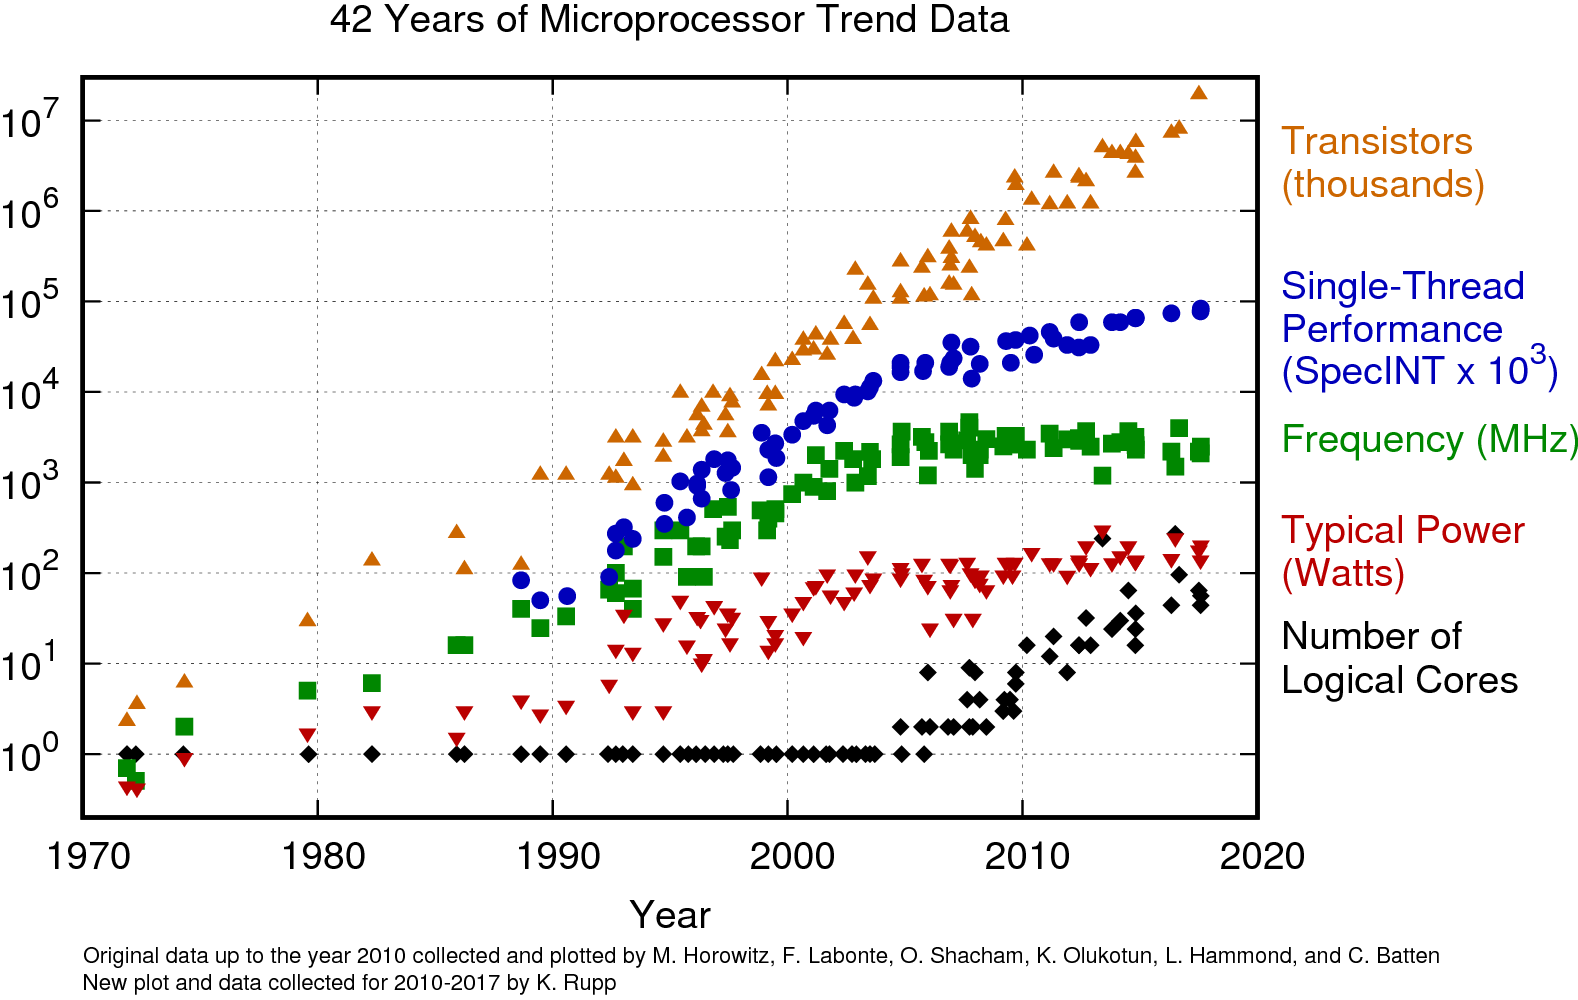
\includegraphics{images/42-years-processor-trend.png}
\caption{trend}
\end{figure}

    \section{Why is can't we go faster?}\label{why-is-cant-we-go-faster}

\begin{itemize}
\tightlist
\item
  Power Management
\item
  Memory~Access Rates
\item
  Instruction Level Parallelism
\end{itemize}

    \section{How to exploit the Sequential Acceleration of CPU and Parallel
Acceleration of
GPU?}\label{how-to-exploit-the-sequential-acceleration-of-cpu-and-parallel-acceleration-of-gpu}

\begin{figure}
\centering
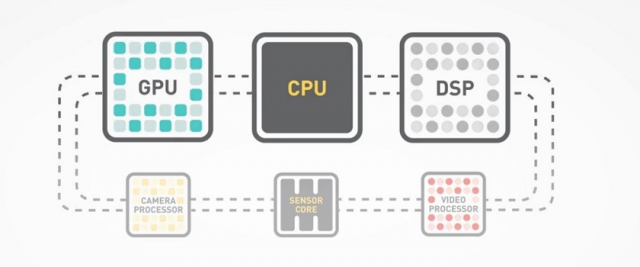
\includegraphics{images/heterogenous_computing.png}
\caption{heterogenous}
\end{figure}

    \section{Heterogenous Computing}\label{heterogenous-computing}

    \section{Basic Idea}\label{basic-idea}

\begin{figure}
\centering
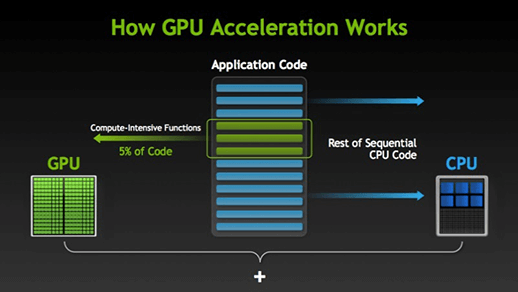
\includegraphics{images/how-gpu-acceleration-works.png}
\caption{basic\_idea}
\end{figure}

    \subsubsection{How does GPU manage to accelerate compute intensive
tasks?}\label{how-does-gpu-manage-to-accelerate-compute-intensive-tasks}

    \begin{itemize}
\tightlist
\item
  Uses parallel programming strategy

  \begin{itemize}
  \tightlist
  \item
    Breaks the tasks into several smaller sub tasks
  \end{itemize}
\end{itemize}

    \begin{itemize}
\tightlist
\item
  Many versions of the sub-tasks operating different data
\end{itemize}

    \begin{itemize}
\tightlist
\item
  Works on the sub tasks simultaneously (parallely).
\end{itemize}

    \subsubsection{How does CPU approach this same
task?}\label{how-does-cpu-approach-this-same-task}

    \begin{itemize}
\tightlist
\item
  Uses single thread. Single stream of instructions.
\end{itemize}

    \begin{itemize}
\tightlist
\item
  Tries to accelerate that single stream of instruction.
\end{itemize}

    \begin{itemize}
\tightlist
\item
  Sequential Processing!
\end{itemize}

    \subsection{\texorpdfstring{What are those
\texttt{tasks}?}{What are those tasks?}}\label{what-are-those-tasks}

    \subsection{Computational tasks}\label{computational-tasks}

    \begin{itemize}
\tightlist
\item
  Matrix Multiplications
\item
  Vector Addition
\item
  Fast Fourier Transforms
\end{itemize}

    \begin{itemize}
\tightlist
\item
  Signal Processing techniques
\item
  Deep Learning Workloads
\end{itemize}

    \subsection{Breaking a task into
sub-tasks}\label{breaking-a-task-into-sub-tasks}

    \begin{itemize}
\tightlist
\item
  Crutial to attain maximum performance
\end{itemize}

    \begin{itemize}
\tightlist
\item
  Depends from task to task
\end{itemize}

    \begin{itemize}
\tightlist
\item
  Some tasks are easier and straight-forward than others
\end{itemize}

    \begin{itemize}
\tightlist
\item
  Lets see an example
\end{itemize}

    \subsection{Vector Addition}\label{vector-addition}

\begin{itemize}
\tightlist
\item
  Vectors are columns of numbers
\end{itemize}

\[\vec{a} = \begin{bmatrix}1 \\2\\\vdots\\n\end{bmatrix}_{n \times 1}\]

    Lets take 2 vectors \(\vec{a}, \vec{b}\) both in \(\mathbb{R}^n\)
(n-dimensional space).

    \begin{equation}
\vec{a} = \begin{bmatrix}a_1 \\a_2\\\vdots\\a_n\end{bmatrix}
\end{equation}

    \begin{equation}
\vec{b} = \begin{bmatrix}b_1 \\b_2\\\vdots\\b_n\end{bmatrix}
\end{equation}

    Whats this quantity? \[\vec{a} + \vec{b}\]

    \begin{itemize}
\tightlist
\item
  Element wise addition
\end{itemize}

\begin{equation}
\vec{a} + \vec{b} = \begin{bmatrix}a_1 + b_1\\a_2+b_2\\a_3+b_3\\\vdots\\a_n+b_n\end{bmatrix}
\end{equation}

    \begin{Verbatim}[commandchars=\\\{\}]
{\color{incolor}In [{\color{incolor} }]:} \PY{k}{for} \PY{n}{i} \PY{o+ow}{in} \PY{n+nb}{range}\PY{p}{(}\PY{n}{n}\PY{p}{)}\PY{p}{:}
            \PY{n}{c}\PY{p}{[}\PY{n}{i}\PY{p}{]} \PY{o}{=} \PY{n}{a}\PY{p}{[}\PY{n}{i}\PY{p}{]} \PY{o}{+} \PY{n}{b}\PY{p}{[}\PY{n}{i}\PY{p}{]}
\end{Verbatim}


    \section{How to split it into sub
tasks?}\label{how-to-split-it-into-sub-tasks}

\begin{quote}
In other words parallelize it?
\end{quote}

    \subsection{Here are the steps (simple
algorithms):}\label{here-are-the-steps-simple-algorithms}

    \begin{itemize}
\tightlist
\item
  Identify independent instructions (operations)
\end{itemize}

    \begin{itemize}
\tightlist
\item
  Identify their input of these indepedent operations
\end{itemize}

    \begin{itemize}
\tightlist
\item
  Finalze your fundamental unit that will have several versions running
  parallely.
\end{itemize}

    \subsection{Revisiting Visiting Vector
Addition}\label{revisiting-visiting-vector-addition}

    \begin{itemize}
\tightlist
\item
  Whats the fundamental operation performed?
\item
  Whats the input for this operation to be performed?
\end{itemize}

    Fundamental Operation: \textbf{Addition of 2 numbers}

Input: One Elements from 2 vectors \textbf{\texttt{a{[}i{]},\ b{[}i{]}}}

    Same operation is performed on different data items. (here
\(a[i], b[i]\))

\begin{quote}
\textbf{SIMD} Processing - \textbf{S}ingle \textbf{I}nstruction
\textbf{M}ultiple \textbf{D}ata Processing
\end{quote}

    \subsubsection{Our Approach to program this addition in
GPU:}\label{our-approach-to-program-this-addition-in-gpu}

    \begin{itemize}
\tightlist
\item
  Replicate \texttt{addition} on different compute units in GPUs
\item
  Give appropriate inputs to these units so that they perform useful
  operation.
\item
  Aggregate the each units output and send it to CPU
\end{itemize}

    \subsection{Terminologies}\label{terminologies}

    \begin{itemize}
\tightlist
\item
  \textbf{Device}: GPU (Device memory: GPU Memory)
\end{itemize}

    \begin{itemize}
\tightlist
\item
  \textbf{Host}: CPU (Host Memory: CPU Memory)
\end{itemize}

    \begin{itemize}
\tightlist
\item
  \textbf{Kernel}: The function that runs in GPU

  \begin{itemize}
  \tightlist
  \item
    Whats our kernel in vector addition?
  \end{itemize}
\end{itemize}

    \begin{itemize}
\tightlist
\item
  \textbf{Threads}: The computational units in GPUs. Runs a version of
  the kernel.
\end{itemize}

    \begin{itemize}
\tightlist
\item
  \textbf{Blocks}: Collections of a set of threads
\end{itemize}

    \begin{itemize}
\tightlist
\item
  \textbf{Grid}: Collection of set of blocks
\end{itemize}

    \subsection{Lets Code Vector Scaling in GPU using
Numba!}\label{lets-code-vector-scaling-in-gpu-using-numba}

    \section{Sample Introduction to
Numba}\label{sample-introduction-to-numba}

Numba gives you the power to speed up your applications with high
performance functions written directly in Python.

We will look into a basic program and understand the Numba~programming
basics.

    \begin{Verbatim}[commandchars=\\\{\}]
{\color{incolor}In [{\color{incolor}1}]:} \PY{c+c1}{\PYZsh{} !conda install \PYZhy{}c numba numba}
        \PY{k+kn}{import} \PY{n+nn}{numba}
\end{Verbatim}


    \begin{Verbatim}[commandchars=\\\{\}]
{\color{incolor}In [{\color{incolor}2}]:} \PY{k+kn}{from} \PY{n+nn}{numba} \PY{k}{import} \PY{n}{cuda}
        \PY{n+nb}{print}\PY{p}{(}\PY{n}{cuda}\PY{o}{.}\PY{n}{gpus}\PY{p}{)}
\end{Verbatim}


    \begin{Verbatim}[commandchars=\\\{\}]
<Managed Device 0>

    \end{Verbatim}

    \begin{Verbatim}[commandchars=\\\{\}]
{\color{incolor}In [{\color{incolor}17}]:} \PY{k+kn}{import} \PY{n+nn}{numpy} \PY{k}{as} \PY{n+nn}{np}
         \PY{c+c1}{\PYZsh{} SCALING A VECTOR BY 2}
         \PY{c+c1}{\PYZsh{} Create the data array \PYZhy{} usually initialized some other way}
         \PY{n}{data} \PY{o}{=} \PY{n}{np}\PY{o}{.}\PY{n}{ones}\PY{p}{(}\PY{l+m+mi}{256}\PY{o}{*}\PY{l+m+mi}{4096}\PY{p}{)} \PY{c+c1}{\PYZsh{} 1,041,664}
         
         \PY{n}{threadsperblock} \PY{o}{=} \PY{l+m+mi}{256}
         
         \PY{c+c1}{\PYZsh{} Ceil function}
         \PY{n}{blockspergrid} \PY{o}{=} \PY{p}{(}\PY{n}{data}\PY{o}{.}\PY{n}{size} \PY{o}{+} \PY{p}{(}\PY{n}{threadsperblock} \PY{o}{\PYZhy{}} \PY{l+m+mi}{1}\PY{p}{)}\PY{p}{)} \PY{o}{/}\PY{o}{/} \PY{n}{threadsperblock}
         \PY{n+nb}{print} \PY{p}{(}\PY{l+s+s2}{\PYZdq{}}\PY{l+s+s2}{Blocks in one grid:}\PY{l+s+se}{\PYZbs{}t}\PY{l+s+s2}{\PYZdq{}} \PY{o}{+} \PY{n+nb}{str}\PY{p}{(}\PY{n}{blockspergrid}\PY{p}{)}\PY{p}{)}
         \PY{n+nb}{print} \PY{p}{(}\PY{l+s+s2}{\PYZdq{}}\PY{l+s+s2}{Threads in one Block:}\PY{l+s+se}{\PYZbs{}t}\PY{l+s+s2}{\PYZdq{}} \PY{o}{+} \PY{n+nb}{str}\PY{p}{(}\PY{n}{threadsperblock}\PY{p}{)}\PY{p}{)}
\end{Verbatim}


    \begin{Verbatim}[commandchars=\\\{\}]
Blocks in one grid:	4096
Threads in one Block:	256

    \end{Verbatim}

    \section{Whats this threadsperblock, blockspergrid
business?}\label{whats-this-threadsperblock-blockspergrid-business}

    \begin{itemize}
\tightlist
\item
  For effective parallelization of higher dimensional data structures,
  loopy data structures:

  \begin{itemize}
  \tightlist
  \item
    CUDA follows an hierarchy
  \item
    threads, blocks, grids we saw remember?
  \end{itemize}
\end{itemize}

    \subsection{Hierarchy}\label{hierarchy}

\begin{itemize}
\tightlist
\item
  \textbf{Threads}: The computational units in GPUs. Runs a version of
  the kernel.
\item
  \textbf{Blocks}: Collections of a set of threads
\item
  \textbf{Grid}: Collection of set of blocks
\end{itemize}

    \subsubsection{We defined how many blocks and threads are
needed.}\label{we-defined-how-many-blocks-and-threads-are-needed.}

\subsubsection{Now lets define the kernel
function}\label{now-lets-define-the-kernel-function}

    \begin{Verbatim}[commandchars=\\\{\}]
{\color{incolor}In [{\color{incolor}18}]:} \PY{k+kn}{from} \PY{n+nn}{numba} \PY{k}{import} \PY{n}{cuda}
         
         \PY{n+nd}{@cuda}\PY{o}{.}\PY{n}{jit}
         \PY{k}{def} \PY{n+nf}{my\PYZus{}kernel}\PY{p}{(}\PY{n}{io\PYZus{}array}\PY{p}{)}\PY{p}{:}
             \PY{n}{pos} \PY{o}{=} \PY{n}{cuda}\PY{o}{.}\PY{n}{grid}\PY{p}{(}\PY{l+m+mi}{1}\PY{p}{)}
             \PY{k}{if} \PY{n}{pos} \PY{o}{\PYZlt{}} \PY{n}{io\PYZus{}array}\PY{o}{.}\PY{n}{size}\PY{p}{:}  \PY{c+c1}{\PYZsh{} Check array boundaries}
                 \PY{n}{io\PYZus{}array}\PY{p}{[}\PY{n}{pos}\PY{p}{]} \PY{o}{*}\PY{o}{=} \PY{l+m+mi}{2} \PY{c+c1}{\PYZsh{} do the computation}
\end{Verbatim}


    \begin{figure}
\centering
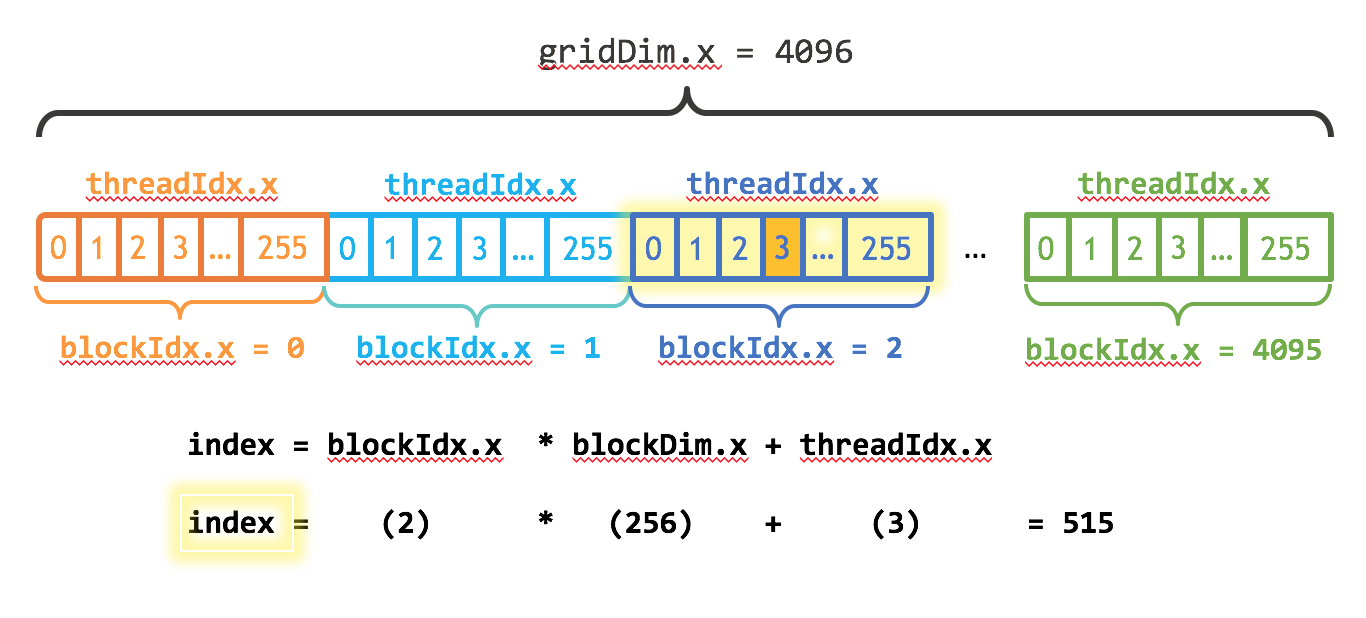
\includegraphics{images/cuda_indexing.png}
\caption{1D\_blocks}
\end{figure}

    \section{Finding the global index of the
thread}\label{finding-the-global-index-of-the-thread}

\begin{itemize}
\tightlist
\item
  \textbf{numba.cuda.grid(ndim)} - Return the absolute position of the
  current thread in the entire grid of blocks.
\end{itemize}

    \subsection{Calling the Kernel from the
code}\label{calling-the-kernel-from-the-code}

    \begin{Verbatim}[commandchars=\\\{\}]
{\color{incolor}In [{\color{incolor}19}]:} \PY{o}{\PYZpc{}\PYZpc{}}\PY{k}{timeit}
         \PYZsh{} Now start the kernel
         \PYZsh{} And time the GPU execution time also
         my\PYZus{}kernel[blockspergrid, threadsperblock](data)
\end{Verbatim}


    \begin{Verbatim}[commandchars=\\\{\}]
13.6 ms ± 66.5 µs per loop (mean ± std. dev. of 7 runs, 100 loops each)

    \end{Verbatim}

    \begin{Verbatim}[commandchars=\\\{\}]
{\color{incolor}In [{\color{incolor}24}]:} \PY{n+nb}{print}\PY{p}{(}\PY{n}{data}\PY{p}{)}
\end{Verbatim}


    \begin{Verbatim}[commandchars=\\\{\}]
[2. 2. 2. {\ldots} 2. 2. 2.]

    \end{Verbatim}

    \begin{Verbatim}[commandchars=\\\{\}]
{\color{incolor}In [{\color{incolor}7}]:} \PY{o}{\PYZpc{}\PYZpc{}}\PY{k}{timeit}
        \PYZsh{} timing the CPU Operations
        data\PYZus{}2 = data*2
\end{Verbatim}


    \begin{Verbatim}[commandchars=\\\{\}]
2.35 ms ± 278 µs per loop (mean ± std. dev. of 7 runs, 100 loops each)

    \end{Verbatim}

    \begin{Verbatim}[commandchars=\\\{\}]
{\color{incolor}In [{\color{incolor}21}]:} \PY{n+nd}{@cuda}\PY{o}{.}\PY{n}{jit}
         \PY{k}{def} \PY{n+nf}{my\PYZus{}kernel2}\PY{p}{(}\PY{n}{io\PYZus{}array}\PY{p}{)}\PY{p}{:}
             \PY{n}{pos} \PY{o}{=} \PY{n}{cuda}\PY{o}{.}\PY{n}{grid}\PY{p}{(}\PY{l+m+mi}{1}\PY{p}{)}
             \PY{k}{if} \PY{n}{pos} \PY{o}{\PYZlt{}} \PY{n}{io\PYZus{}array}\PY{o}{.}\PY{n}{size}\PY{p}{:}
                 \PY{n}{io\PYZus{}array}\PY{p}{[}\PY{n}{pos}\PY{p}{]} \PY{o}{*}\PY{o}{=} \PY{l+m+mi}{2} \PY{c+c1}{\PYZsh{} do the computation}
\end{Verbatim}


    \begin{Verbatim}[commandchars=\\\{\}]
{\color{incolor}In [{\color{incolor}22}]:} \PY{c+c1}{\PYZsh{} Host code   }
         \PY{n}{data} \PY{o}{=} \PY{n}{np}\PY{o}{.}\PY{n}{ones}\PY{p}{(}\PY{l+m+mi}{256}\PY{o}{*}\PY{l+m+mi}{4096}\PY{p}{)}
         \PY{n}{threadsperblock} \PY{o}{=} \PY{l+m+mi}{256}
         \PY{n}{blockspergrid} \PY{o}{=} \PY{n}{np}\PY{o}{.}\PY{n}{ceil}\PY{p}{(}\PY{n}{data}\PY{o}{.}\PY{n}{shape}\PY{p}{[}\PY{l+m+mi}{0}\PY{p}{]} \PY{o}{/} \PY{n}{threadsperblock}\PY{p}{)}\PY{o}{.}\PY{n}{astype}\PY{p}{(}\PY{l+s+s1}{\PYZsq{}}\PY{l+s+s1}{int32}\PY{l+s+s1}{\PYZsq{}}\PY{p}{)}
         \PY{n}{my\PYZus{}kernel2}\PY{p}{[}\PY{n}{blockspergrid}\PY{p}{,} \PY{n}{threadsperblock}\PY{p}{]}\PY{p}{(}\PY{n}{data}\PY{p}{)}
\end{Verbatim}


    \begin{Verbatim}[commandchars=\\\{\}]
{\color{incolor}In [{\color{incolor}23}]:} \PY{n+nb}{print}\PY{p}{(}\PY{n}{data}\PY{p}{)}
\end{Verbatim}


    \begin{Verbatim}[commandchars=\\\{\}]
[2. 2. 2. {\ldots} 2. 2. 2.]

    \end{Verbatim}

    \section{Lets do Matrix Multiplication in
GPU!}\label{lets-do-matrix-multiplication-in-gpu}

\begin{quote}
How will you approach this problem????
\end{quote}

\begin{quote}
How will you assign the threads and blocks?
\end{quote}

    \begin{figure}
\centering
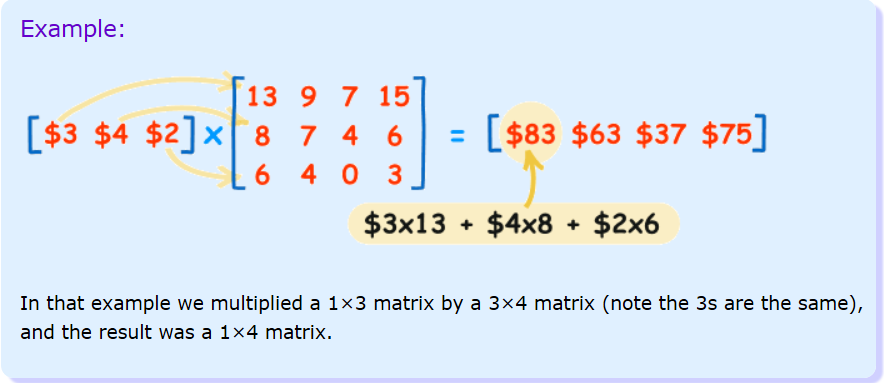
\includegraphics{images/matmul.png}
\caption{matrix\_mul}
\end{figure}

    \subsection{Remember the guidelines:}\label{remember-the-guidelines}

\begin{itemize}
\tightlist
\item
  Identify independent instructions (operations)
\item
  Identify their input of these indepedent operations
\item
  Finalize your fundamental unit that will have several versions running
  parallely.
\end{itemize}

    \begin{figure}
\centering
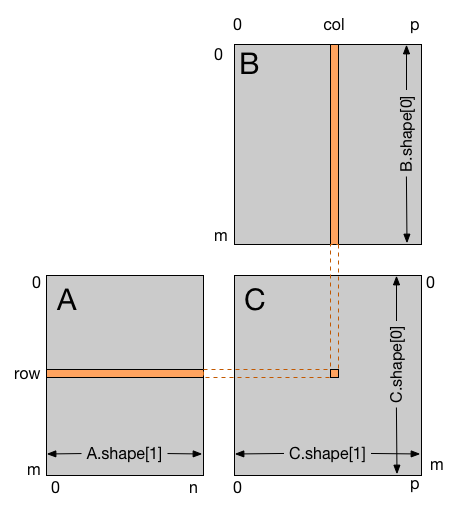
\includegraphics{images/05-matmul.png}
\caption{matrix}
\end{figure}

    \subsection{What's the dimension of the block
here?}\label{whats-the-dimension-of-the-block-here}

\begin{quote}
Is it 1D as we saw in scalar multiplication?
\end{quote}

    \begin{figure}
\centering
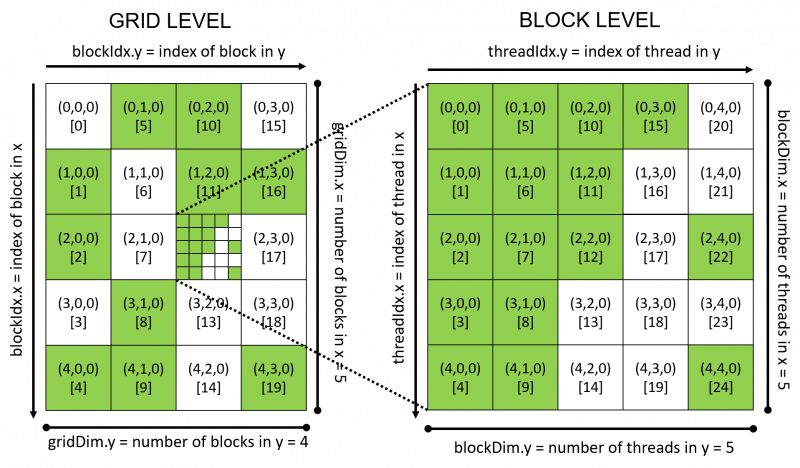
\includegraphics{images/blocksmatmul.png}
\caption{image}
\end{figure}

    \begin{figure}
\centering
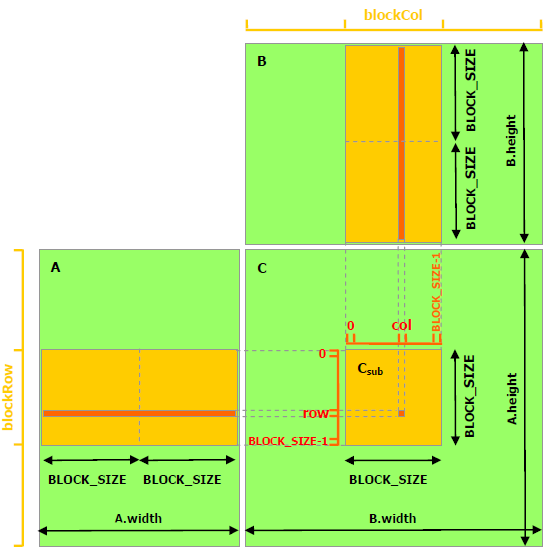
\includegraphics{images/tile.png}
\caption{image}
\end{figure}

    \section{Lets code this in Numba}\label{lets-code-this-in-numba}

    \subsubsection{Host Code}\label{host-code}

    \begin{Verbatim}[commandchars=\\\{\}]
{\color{incolor}In [{\color{incolor}26}]:} \PY{c+c1}{\PYZsh{} Host code}
         
         \PY{c+c1}{\PYZsh{} Initialize the data arrays}
         \PY{n}{m} \PY{o}{=} \PY{l+m+mi}{2}\PY{o}{*}\PY{o}{*}\PY{l+m+mi}{11} \PY{c+c1}{\PYZsh{} 2048}
         \PY{n}{n} \PY{o}{=} \PY{l+m+mi}{2}\PY{o}{*}\PY{o}{*}\PY{l+m+mi}{11}
         \PY{n}{p} \PY{o}{=} \PY{l+m+mi}{2}\PY{o}{*}\PY{o}{*}\PY{l+m+mi}{11}
         
         \PY{n}{A} \PY{o}{=} \PY{n}{np}\PY{o}{.}\PY{n}{full}\PY{p}{(}\PY{p}{(}\PY{n}{m}\PY{p}{,} \PY{n}{n}\PY{p}{)}\PY{p}{,} \PY{l+m+mi}{1}\PY{p}{,} \PY{n}{np}\PY{o}{.}\PY{n}{float}\PY{p}{)} \PY{c+c1}{\PYZsh{} matrix containing all 1\PYZsq{}s}
         \PY{n}{B} \PY{o}{=} \PY{n}{np}\PY{o}{.}\PY{n}{full}\PY{p}{(}\PY{p}{(}\PY{n}{n}\PY{p}{,} \PY{n}{p}\PY{p}{)}\PY{p}{,} \PY{l+m+mi}{1}\PY{p}{,} \PY{n}{np}\PY{o}{.}\PY{n}{float}\PY{p}{)} \PY{c+c1}{\PYZsh{} matrix containing all 1\PYZsq{}s}
\end{Verbatim}


    \subsubsection{Host to device data transfer + Memory allocation in
GPU}\label{host-to-device-data-transfer-memory-allocation-in-gpu}

    \begin{Verbatim}[commandchars=\\\{\}]
{\color{incolor}In [{\color{incolor}27}]:} \PY{c+c1}{\PYZsh{} Copy the arrays to the device}
         \PY{n}{A\PYZus{}global\PYZus{}mem} \PY{o}{=} \PY{n}{cuda}\PY{o}{.}\PY{n}{to\PYZus{}device}\PY{p}{(}\PY{n}{A}\PY{p}{)}
         \PY{n}{B\PYZus{}global\PYZus{}mem} \PY{o}{=} \PY{n}{cuda}\PY{o}{.}\PY{n}{to\PYZus{}device}\PY{p}{(}\PY{n}{B}\PY{p}{)}
         
         \PY{c+c1}{\PYZsh{} Allocate memory on the device for the result}
         \PY{n}{C\PYZus{}global\PYZus{}mem} \PY{o}{=} \PY{n}{cuda}\PY{o}{.}\PY{n}{device\PYZus{}array}\PY{p}{(}\PY{p}{(}\PY{n}{m}\PY{p}{,} \PY{n}{p}\PY{p}{)}\PY{p}{)}
\end{Verbatim}


    \subsection{Kernel}\label{kernel}

    \begin{Verbatim}[commandchars=\\\{\}]
{\color{incolor}In [{\color{incolor}28}]:} \PY{n+nd}{@cuda}\PY{o}{.}\PY{n}{jit}
         \PY{k}{def} \PY{n+nf}{matmul}\PY{p}{(}\PY{n}{A}\PY{p}{,} \PY{n}{B}\PY{p}{,} \PY{n}{C}\PY{p}{)}\PY{p}{:}
             \PY{l+s+sd}{\PYZdq{}\PYZdq{}\PYZdq{}Perform matrix multiplication of C = A * B}
         \PY{l+s+sd}{    \PYZdq{}\PYZdq{}\PYZdq{}}
             \PY{n}{i}\PY{p}{,} \PY{n}{j} \PY{o}{=} \PY{n}{cuda}\PY{o}{.}\PY{n}{grid}\PY{p}{(}\PY{l+m+mi}{2}\PY{p}{)}
             \PY{k}{if} \PY{n}{i} \PY{o}{\PYZlt{}} \PY{n}{C}\PY{o}{.}\PY{n}{shape}\PY{p}{[}\PY{l+m+mi}{0}\PY{p}{]} \PY{o+ow}{and} \PY{n}{j} \PY{o}{\PYZlt{}} \PY{n}{C}\PY{o}{.}\PY{n}{shape}\PY{p}{[}\PY{l+m+mi}{1}\PY{p}{]}\PY{p}{:}
                 \PY{n}{tmp} \PY{o}{=} \PY{l+m+mf}{0.}
                 \PY{k}{for} \PY{n}{k} \PY{o+ow}{in} \PY{n+nb}{range}\PY{p}{(}\PY{n}{A}\PY{o}{.}\PY{n}{shape}\PY{p}{[}\PY{l+m+mi}{1}\PY{p}{]}\PY{p}{)}\PY{p}{:}
                     \PY{n}{tmp} \PY{o}{+}\PY{o}{=} \PY{n}{A}\PY{p}{[}\PY{n}{i}\PY{p}{,} \PY{n}{k}\PY{p}{]} \PY{o}{*} \PY{n}{B}\PY{p}{[}\PY{n}{k}\PY{p}{,} \PY{n}{j}\PY{p}{]}
                 \PY{n}{C}\PY{p}{[}\PY{n}{i}\PY{p}{,} \PY{n}{j}\PY{p}{]} \PY{o}{=} \PY{n}{tmp}
\end{Verbatim}


    \subsection{Defining threadsperblock,
blockspergrid}\label{defining-threadsperblock-blockspergrid}

    \begin{Verbatim}[commandchars=\\\{\}]
{\color{incolor}In [{\color{incolor}29}]:} \PY{n}{threadsperblock} \PY{o}{=} \PY{p}{(}\PY{l+m+mi}{32}\PY{p}{,} \PY{l+m+mi}{32}\PY{p}{)}
         \PY{c+c1}{\PYZsh{} Dimension of the matrix we defined is 2048x2048}
\end{Verbatim}


    \begin{Verbatim}[commandchars=\\\{\}]
{\color{incolor}In [{\color{incolor}30}]:} \PY{n}{blockspergrid\PYZus{}x} \PY{o}{=} \PY{n+nb}{int}\PY{p}{(}\PY{n}{np}\PY{o}{.}\PY{n}{ceil}\PY{p}{(}\PY{n}{A}\PY{o}{.}\PY{n}{shape}\PY{p}{[}\PY{l+m+mi}{0}\PY{p}{]} \PY{o}{/} \PY{n}{threadsperblock}\PY{p}{[}\PY{l+m+mi}{0}\PY{p}{]}\PY{p}{)}\PY{p}{)}
         \PY{n}{blockspergrid\PYZus{}y} \PY{o}{=} \PY{n+nb}{int}\PY{p}{(}\PY{n}{np}\PY{o}{.}\PY{n}{ceil}\PY{p}{(}\PY{n}{B}\PY{o}{.}\PY{n}{shape}\PY{p}{[}\PY{l+m+mi}{1}\PY{p}{]} \PY{o}{/} \PY{n}{threadsperblock}\PY{p}{[}\PY{l+m+mi}{1}\PY{p}{]}\PY{p}{)}\PY{p}{)}
         \PY{n}{blockspergrid} \PY{o}{=} \PY{p}{(}\PY{n}{blockspergrid\PYZus{}x}\PY{p}{,} \PY{n}{blockspergrid\PYZus{}y}\PY{p}{)}
\end{Verbatim}


    \subsection{Kernel Call}\label{kernel-call}

    \begin{Verbatim}[commandchars=\\\{\}]
{\color{incolor}In [{\color{incolor}31}]:} \PY{c+c1}{\PYZsh{} Start the kernel }
         \PY{n}{matmul}\PY{p}{[}\PY{n}{blockspergrid}\PY{p}{,} \PY{n}{threadsperblock}\PY{p}{]}\PY{p}{(}\PY{n}{A\PYZus{}global\PYZus{}mem}\PY{p}{,} \PY{n}{B\PYZus{}global\PYZus{}mem}\PY{p}{,} \PY{n}{C\PYZus{}global\PYZus{}mem}\PY{p}{)}
         
         \PY{c+c1}{\PYZsh{} Copy the result back to the host}
         \PY{n}{C} \PY{o}{=} \PY{n}{C\PYZus{}global\PYZus{}mem}\PY{o}{.}\PY{n}{copy\PYZus{}to\PYZus{}host}\PY{p}{(}\PY{p}{)}
\end{Verbatim}


    \begin{Verbatim}[commandchars=\\\{\}]
{\color{incolor}In [{\color{incolor}32}]:} \PY{n+nb}{print}\PY{p}{(}\PY{n}{C}\PY{p}{)}
\end{Verbatim}


    \begin{Verbatim}[commandchars=\\\{\}]
[[2048. 2048. 2048. {\ldots} 2048. 2048. 2048.]
 [2048. 2048. 2048. {\ldots} 2048. 2048. 2048.]
 [2048. 2048. 2048. {\ldots} 2048. 2048. 2048.]
 {\ldots}
 [2048. 2048. 2048. {\ldots} 2048. 2048. 2048.]
 [2048. 2048. 2048. {\ldots} 2048. 2048. 2048.]
 [2048. 2048. 2048. {\ldots} 2048. 2048. 2048.]]

    \end{Verbatim}

    \section{Lets time it!}\label{lets-time-it}

    \begin{Verbatim}[commandchars=\\\{\}]
{\color{incolor}In [{\color{incolor}33}]:} \PY{o}{\PYZpc{}\PYZpc{}}\PY{k}{timeit} \PYZhy{}n 10
         matmul[blockspergrid, threadsperblock](A\PYZus{}global\PYZus{}mem, B\PYZus{}global\PYZus{}mem, C\PYZus{}global\PYZus{}mem)
\end{Verbatim}


    \begin{Verbatim}[commandchars=\\\{\}]
299 µs ± 134 µs per loop (mean ± std. dev. of 7 runs, 10 loops each)

    \end{Verbatim}

    \begin{Verbatim}[commandchars=\\\{\}]
{\color{incolor}In [{\color{incolor}34}]:} \PY{o}{\PYZpc{}\PYZpc{}}\PY{k}{timeit} \PYZhy{}n 10
         C = A.dot(B)
\end{Verbatim}


    \begin{Verbatim}[commandchars=\\\{\}]
463 ms ± 20.4 ms per loop (mean ± std. dev. of 7 runs, 10 loops each)

    \end{Verbatim}

    \section{New Moore's Law}\label{new-moores-law}

\begin{itemize}
\item
  Computers no longer get faster, just Wider
\item
  Rethink your algorithms to be parallel
\item
  Data-Parallel Computing is the most scalable solution
\end{itemize}

    \begin{figure}
\centering
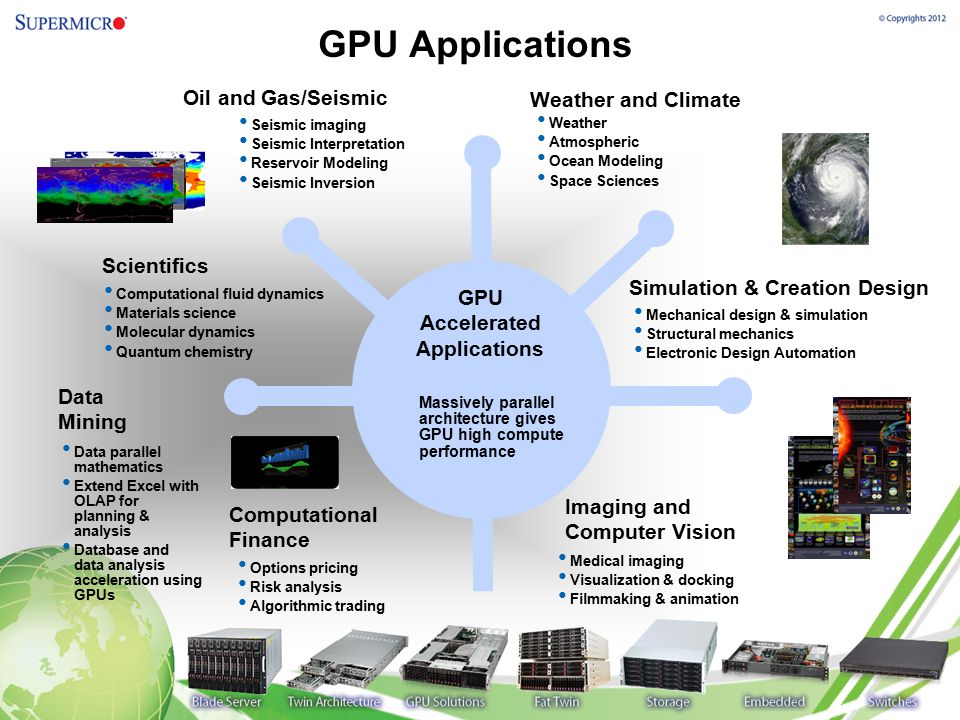
\includegraphics{images/GPU+Accelerated+Applications.jpg}
\caption{gpu-applications}
\end{figure}

    \section{Summary}\label{summary}

    \subsection{Thanks for your patience}\label{thanks-for-your-patience}

This presentation and extensive resources can be found in my GitHub -
\href{github.com/tlokeshkumar}{tlokeshkumar}.

Even projects and other codes in GPU Programming, Deep Learning etc are
present in my GitHub.... Do check them out if interested!!!

Feel free to contact me at lokesh.karpagam@gmail.com


    % Add a bibliography block to the postdoc
    
    
    
    \end{document}
